\chapter{Introducci\'on}

En la neurociencia moderna existe la teor\'ia de que el cerebro
puede ser dividido en \'areas de acuerdo a distintos criterios
estructurales, siendo la citoarquitectura de Broadmann \cite{Brodmann1909}
una de la m\'as conocidas. Actualmente existe evidencia de que es posible
atribuir un criterio funcional a cada una de estas regiones, como mover la
mano o procesar el lenguaje \cite{Greicius2003}. No obstante, el c\'omo se
relacionan dichas \'areas con funciones complejas sigue siendo un problema
abierto \cite{Barch2013}. As\'i mismo, tampoco se conoce si esta divisi\'on
es \'unica, y en tal caso, qu\'e l\'imites definen a cada \'area. La
relaci\'on funci\'on-estructura posee diversas aplicaciones en la
medicina, como por ejemplo el planeamiento quir\'urgico 
\cite{Stufflebeam2011} \cite{Oishi2010}; asistencia durante la cirug\'ia
\cite{DeSchotten2005} y rehabilitaci\'on \cite{Song2014} de pacientes. 
Por ello existe la necesidad de entender c\'omo es que el cerebro est\'a
conectado estructuralmente, esto es, entender qu\'e regiones est\'an
conectadas f\'isicamente por axones y cu\'anto influye esto en el aspecto
funcional del cerebro. \\

El cerebro puede dividirse en varios tipos de tejido, nosotros nos
enfocaremos en dos de ellos: materia blanca y materia gris. La corteza 
est\'a formada por materia gris, la cual es densa en neuronas. Estas
neuronas est\'an conectadas entre si mediante axones. Se denomina materia
blanca al tejido donde la proporci\'on de axones es superior a la de
neuronas \cite{Dale2008}. La reciente invenci\'on de la Resonancia 
Magn\'etica de Difusi\'on (dMRI) permiti\'o desarrollar nuevas t\'ecnicas
para estudiar la conectividad estructural \cite{Taylor1985}. En
particular, el conocer la intensidad de difusi\'on que existe en cada
punto del cerebro permite caracterizar los axones dentro de la materia
blanca \cite{Hagmann2006}. Una forma de hacerlo es utilizando algoritmos
de tractograf\'ia \cite{Descoteaux2009, Jbabdi2007}, estos toman un
punto del cerebro como semilla y devuelven un tractograma. Un tractograma
es una imagen donde cada voxel representa la probabilidad de que ese punto
del cerebro est\'e conectado a la semilla elegida mediante un conjunto de
axones. Las probabilidades se estiman mediante un procedimiento Monte
Carlo, simulando el recorrido de un n\'umero de part\'iculas de agua por
la materia blanca comenzando desde dicha semilla. Distintos grupos han
propuesto el agrupar semillas para definir nuevos criterios de
parcelamiento de la corteza cerebral. Esto se puede hacer empleando algoritmos de \textit{clustering} sobre los tractogramas de las semillas.\\

Los algoritmos de \textit{clustering} son herramientas de an\'alisis en
campos como \textit{Machine Learning} y \textit{Data Mining}. Permiten
clasificar objetos en base a distintos criterios. Ejemplos de ellos son: 

\begin{itemize}
    \item K-means \cite{Hartigan1979}: Divide $n$ vectores en $k$ clusters
                   diferentes, siendo
                   $k$ un n\'umero predefinido. Cada cluster est\'a
                   formado por los elementos que m\'as cerca est\'an al
                   vector medio del cluster.
    \item Agglomerative Hierarchical Clustering \cite{Mining2009}:
                   Cada observaci\'on
                   comienza en un $cluster$ distinto. Luego, iterativamente
                   el algoritmo selecciona dos clusters siguiendo alg\'un
                   criterio de similitud, los agrupa en un nuevo $cluster$ 
                   y crea un elemento representativo de este. El proceso
                   finaliza cuando solo queda un $cluster$. La jerarqu\'ia
                   resultante de agrupar todos los $clusters$ es expresada
                   mediante un dendrograma .
    \item Gaussian Mixture \cite{Mining2009}: Asume que todas las
                   observaciones provienen de
                   un n\'umero finito de distribuciones Gaussianas con 
                   par\'ametros desconocidos. Implementa 
                   \textit{expectation-maximization} para determinar
                   dichos par\'ametros iterativamente.
\end{itemize}

Cada algoritmo utiliza distintos modelos de $cluster$, por lo que el
espacio de aplicaci\'on y el resultado var\'ia significativamente de uno a
otro. \\

\begin{wrapfigure}{r}{0.5\textwidth}
    \centering
    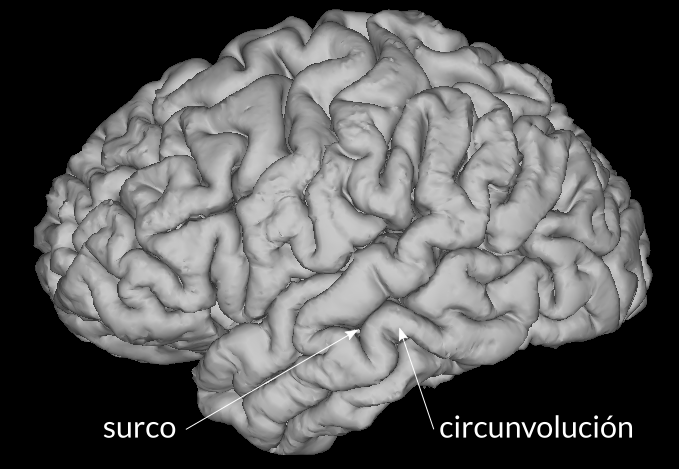
\includegraphics[width=0.5\textwidth]{img/cerebro.png}
    \caption{La corteza cerebral est\'a compuesta por surcos y
             circunvoluciones.}
    \label{fig:cerebro}
\end{wrapfigure}

Para poder parcelar la corteza cerebral mediante el $clustering$ de 
tractogramas es necesario seguir una serie de pasos. El primer paso es
seleccionar la posici\'on de las semillas de cada tractograma. Como la
materia blanca est\'a compuesta principalmente por axones, es en ella
donde se sit\'uan las semillas. Por ello, seleccionar los voxels que 
ser\'an semilla requiere contar con alguna manera de discriminar
entre materia blanca y materia gris. Si ademas queremos que las
semillas est\'en a cierta distancia de la corteza debemos tener cuidado.
La corteza del cerebro no es uniforme, est\'a llena de surcos y 
circunvoluciones como puede verse en la figura \ref{fig:cerebro}.
El segundo paso es generar los tractogramas. En la literatura actual se
utilizan hasta veinte mil semillas por hemisferio 
\cite{Moreno-Dominguez2014} y cien mil part\'iculas por semilla 
\cite{Anwander2006} para generar los tractogramas. Realizar cada
tractograma en paralelo reduce el tiempo total del procesamiento del
cerebro. Al momento de representarlos es importante seleccionar la
estructura correcta. Una matriz del tama\~no de la imagen de dMRI es la
implementaci\'on m\'as sencilla pero, como explicaremos en la secci\'on 
\ref{sec:ralas}, desperdicia mucho espacio. En tercer lugar, para agrupar
los tractogramas se debe seleccionar un modelo para los datos; un
algoritmo de \textit{clustering} y una medida de similaridad. Finalmente,
una vez obtenidos los clusters, es necesario mapear cada semilla con su
respectivo voxel en la corteza cerebral. En resumen, primero hay 
que situar las semillas en la materia blanca; luego se deben generar los 
tractogramas de estas y finalmente hay que aplicar un algoritmo de
\textit{clustering}. \\
 
Dada la cantidad de herramientas disponibles, distintos grupos han
aplicado diferentes criterios de \textit{clustering} para parcelar la
corteza. Por ejemplo, Behrens et. al \cite{Behrens2003} utilizan 
\textit{Target-Based Clustering}. Este algoritmo define como restricci\'on
que cada parcela solo puede estar conectada con alguna otra perteneciente
a un conjunto predefinido. Anwander et. al \cite{Anwander2006} dividen el
\'area de Broca utilizando \textit{k-means}, por lo cual necesitan 
predefinir el n\'umero de parcelas a encontrar. Moreno-Dominguez et al. 
\cite{Moreno-Dominguez2014} utilizan el algoritmo $Agglomerative$
$Hierarchical$ $Clustering$ para parcelar la corteza cerebral. Eligen 
como medida de similitud la distancia coseno y como representante al
centroide. La gran ventaja de este \'ultimo m\'etodo de $clustering$ es
que posee pocas restricciones. No se deben elegir $a priori$ el n\'umero
de parcelas a generar o la forma en que estas deber\'ian estar conectadas.
A su vez, el elegir como cortar el dendrograma permite controlar la
granularidad de la parcelaci\'on. Sin embargo, no queda claro
que el criterio utilizado por Moreno-Dominguez para medir distancias entre
clusters y la forma de representar la uni\'on de los mismos sean
compatibles. Entonces, si bien el m\'etodo de Moreno-Dominguez no asume
cuantas o como son las \'areas a encontrar, a\'un no posee el suficiente
formalismo. Por esto es importante seguir investigando nuevos modelos.  \\

El objetivo de este trabajo es analizar los m\'etodos de 
\textit{clustering} jer\'arquico actuales para parcelar toda la corteza y
proponer un nuevo enfoque. Utilizamos la base de datos provista por 
\textit{Human Connectome Project} \cite{VanEssen2012}. \'Esta posee la
dMRI de varios sujetos organizada por sexo y edad, con la ventaja de que
todos los datos est\'an ya preprocesados. Usar dicha base de datos nos
permite enfocarnos en el problema del \textit{clustering}. A su vez, 
permite reproducir con mayor facilidad nuestro estudio. \\

Una contribuci\'on menor de este trabajo es an\'alizar la implementaci\'on 
existente del algoritmo de tractograf\'ia que usamos. Dada la naturaleza
estoc\'astica del mismo es importante comprobar si el resultado se
estabiliza al utilizar un n\'umero suficientemente grande de semillas. En
particular mostramos que para mas de dos mil particulas los tractogramas
convergen a un mismo resultado. \\

La contribuci\'on principal de este estudio es el realizar un an\'alisis
te\'orico del m\'etodo de Moreno-Dominguez \cite{Moreno-Dominguez2014};
mostrar las problem\'aticas que presenta y proponer una nueva forma de
parcelar la corteza mediante el \textit{clustering} de semillas. Nuestro 
m\'etodo consiste en transformar los tractogramas a un espacio vectorial
y luego agruparlos con \textit{Agglomerative Hierarchical Clustering}. Utilizamos la m\'etrica euclidiana como medida de similitud y el centroide
como \textit{linkage}. Presentamos una implementaci\'on eficiente de
nuestro m\'etodo as\'i como tambi\'en el como adaptarlo al uso de matrices
ralas para optimizar el costo espacial. Mostramos que nuestro algoritmo
produce parcelaciones similares a las obtenidas usando el estado
del arte. La ventaja de nuestro algoritmo es que reduce significativamente
el orden de complejidad temporal y espacial. Tambi\'en mostramos que
nuestros resultados poseen consistencia con parcelaciones anat\'omicas
\cite{Desikan2006} y funcionales  \cite{Barch2013, Penfield1954}, de la
literatura.  \\

Este trabajo est\'a dividido en 6 cap\'itulos. El cap\'itulo 
\ref{ch:bkgrnd} es una breve introducci\'on te\'orica a la Resonancia 
Magn\'etica y a la Resonancia Magn\'etica de Difusi\'on. El cap\'itulo
\ref{ch:metodos} detalla los pasos necesarios a seguir para parcelar la
corteza cerebral usando el m\'etodo de Moreno-Dominguez. El cap\'itulo
\ref{ch:contribuciones} presenta nuestras contribuciones: Explicamos el
algoritmo de tractograf\'ia implementado y como estudiar su estabilidad;
hacemos un analisis te\'orico del m\'etodo de Moreno-Dominguez 
mostrando algunas de sus limitaciones; introducimos una transformaci\'on 
de los tractogramas que nos permite superar las limitaciones de 
Moreno-Dominguez y presentamos nuestro m\'etodo de parcelaci\'on en
detalle. El cap\'itulo \ref{ch:resultados} muestra los resultados de
parcelar el \'area de Broca y la corteza cerebral con ambos m\'etodos.
Finalmente el capitulo \ref{ch:discusion} presenta la discusi\'on de los
resultados obtenidos junto con ideas para futuros trabajos.






